\documentclass{article}

% Generic conference style. Use [final] to show author names.
\usepackage[final]{positionpaper}

\usepackage[utf8]{inputenc}
\usepackage[round,authoryear]{natbib}
\usepackage{hyperref}
\usepackage{url}
\usepackage{booktabs}
\usepackage{tabularx}
\usepackage{amsmath,amssymb,amsthm}
\usepackage{nicefrac}
\usepackage{graphicx}
\usepackage{xcolor}
\usepackage{enumitem}

\newcommand{\note}[1]{\textcolor{red}{#1}}

\hypersetup{colorlinks=true,linkcolor=teal!70!black,citecolor=teal!70!black,urlcolor=teal!70!black}
\graphicspath{{figures/}}

% Let pages end naturally instead of stretching the space between paragraphs.
\raggedbottom
\setlength{\textfloatsep}{12pt plus 2pt minus 2pt}
\setlength{\floatsep}{10pt plus 2pt minus 2pt}

\theoremstyle{definition}
\newtheorem{definition}{Definition}
\theoremstyle{plain}
\newtheorem{proposition}{Proposition}
\theoremstyle{remark}
\newtheorem*{remark}{Remark}
\newcommand{\comp}{\mathrm{comp}}
\newcommand{\rep}{\mathrm{rep}}
\newcommand{\R}{\mathbb{R}}
\newcolumntype{Y}{>{\raggedright\arraybackslash}X}
\newcolumntype{P}[1]{>{\raggedright\arraybackslash}p{#1}}
\setlist{itemsep=1pt,topsep=3pt,parsep=0pt}

\title{Distinguishing Representational and Behavioral\\ Compositionality via Recoverability}

\author{Karthik Singaravadivelan\\ College of Computing, Georgia Institute of Technology}

\begin{document}
\maketitle

\begin{abstract}
Compositionality is believed to be central to intelligence, and
machine learning now applies the term to nearly any successful
recombination of familiar material. Recent work has separated
behavioral evidence for compositionality from representational
evidence, but it has left open what a representation must be like to
count as compositional. In this paper, we propose an answer: a
representation is compositional when it combines parts through a
relation from which every part can be recovered, in its role, by the
same procedure. We show that this criterion accounts for the
properties that Fodor and Pylyshyn attributed to compositional
thought. Systematicity and productivity follow necessarily from a
relation that is separable and invertible, but only contingently from
blending, the mode of combination that neural networks mostly exhibit,
because a blend maps infinitely many combinations of parts onto each
composite. We then describe a suite of tests that distinguishes
recoverability guaranteed by a relation from recoverability borrowed
from a familiar vocabulary, a reference profile of human performance
drawn from the literature, and a plan for evaluating simple neural
networks and existing structured systems against it.
\end{abstract}

%=====================================================================
\section{Introduction}
\label{sec:intro}

Compositionality is among the oldest ideas in the study of mind and
language. \citet{frege1923} observed that we understand sentences we
have never heard because we can build the sense of a sentence from
parts that correspond to its words, and \citet{fodor1988} later argued
that the systematicity and productivity of human thought are explained
by representations with constituent structure. In machine learning,
the idea appears as {\it compositional generalization\/}, the ability
to produce correct outputs for novel combinations of familiar atoms
\citep{lake2018,keysers2020}. Researchers describe text-to-image models
as composing concepts into new scenes \citep{ramesh2021,okawa2023} and
language models as reasoning compositionally \citep{press2023}, yet the
same models often fail to place objects in requested relations
\citep{conwell2022} and express an attribute named for one object on
another \citep{rassin2022}.

Most uses of the term rest on a colloquial definition that descends
from Frege and \citet{montague1970}:

\begin{definition}[Compositionality, colloquial]
\label{def:colloquial}
A system is compositional if the meaning or representation of a
complex expression is determined by the meanings or representations of
its parts and the way in which they are combined.
\end{definition}

\noindent
This definition is satisfied by any system that computes a function of
its inputs, and so it cannot distinguish the two images in
Figure~\ref{fig:ops}. \citet{vegner2025} took a first step by separating
two kinds of evidence, which we state as follows:

\begin{definition}[Behavioral compositionality]
\label{def:behavioral}
Behavioral compositionality is the capacity to produce appropriate
outputs for combinations of familiar parts that a system has not
encountered together, whatever internal process produces those
outputs.
\end{definition}

\begin{definition}[Representational compositionality, informal]
\label{def:representational}
Representational compositionality is the property of a system whose
representation of each composite is built from the representations of
its parts by a relation that is shared across combinations, and from
which each part can be recovered in its role.
\end{definition}

\noindent
\citet{vegner2025} show that behavior does not establish the second
kind, but they leave its criterion to future work in mechanistic
interpretability. \citet{elmoznino2024} define representational
compositionality instead by the simplicity of a symbolic redescription.
Here we propose that the criterion is {\it recoverability\/}, a notion
we take from \citet{vangelder1990}, who called a representation
functionally compositional when general and reliable processes
construct it from its parts and decode it back into them.

\begin{figure}[t]
  \centering
  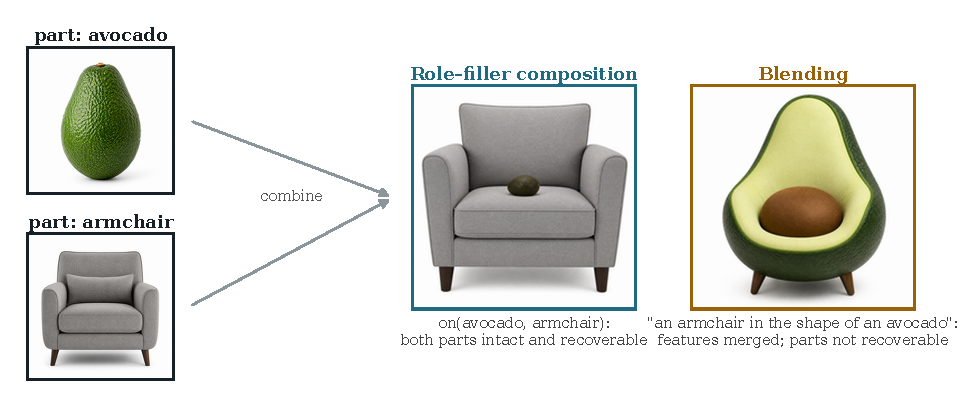
\includegraphics[width=\linewidth]{fig1_avocado.pdf}
  \caption{Two modes of combining the same parts. Role--filler composition places the avocado in a role of the relation \emph{on}, so that both parts remain intact and either can be read back from the whole. Blending merges the features of the two concepts into an armchair in the shape of an avocado, a prompt made familiar by DALL$\cdot$E \citep{openai2021dalle}, from which neither part can be recovered. All four images were generated for this paper with Canva's text-to-image tool.}
  \label{fig:ops}
\end{figure}

Recoverability is central to the classical account in a way that is
easy to miss. \citet{fodor1990} did not deny that a network could behave
systematically. They argued that it would do so only contingently, as
a result of its training, whereas a system with constituent structure
must do so as a matter of its architecture. We adopt their targets,
systematicity and productivity as necessary properties, together with
van Gelder's criterion, and we argue that the necessity comes from the
relation rather than from the tokening of constituents. If one
invertible relation serves every filler and every role, then the
ability to build and decode any composite follows from the ability to
build and decode one. People appear to have such a relation. They
blend concepts, but they also encode agent and patient in separate
codes \citep{frankland2015}, apply a new word in combinations they
have never seen \citep{lake2019}, and draw inferences that depend on
the form of a premise rather than its content \citep{rips1994}.

\textbf{Contributions.} This paper makes three contributions.
\begin{itemize}
  \item A recoverability-based definition of representational
  compositionality, stated over the separability and invertibility of
  the combining relation, with a taxonomy of modes of combination
  (Section~\ref{sec:definition}).
  \item Formal results showing that the definition accounts for
  systematicity, productivity, and the independence of a part from the
  contexts in which it was learned, and that blending supplies none of
  these (Section~\ref{sec:consequences}).
  \item A suite of tests, a human reference profile, and a plan for
  evaluating simple networks and existing structured systems, which
  together determine which mode of combination a system uses
  (Section~\ref{sec:tests}).
\end{itemize}

%=====================================================================
\section{Background}
\label{sec:background}

In this section, we review the four literatures that shaped the term,
emphasizing the role of recoverability in each, and then describe the
problems that arise when its two senses share one name.

\paragraph{Philosophy.} \citet{montague1970} made the Fregean principle
precise by treating syntax and semantics as algebras linked by a
homomorphism. In this form, the principle names a mode of combination
without saying which one. \citet{fodor1988} responded to the
connectionist models of the 1980s \citep{rumelhart1986} with an
argument in three steps. Human thought is productive and systematic.
Both properties follow if representations have constituent structure
that structure-sensitive operations can use. A network without such
structure cannot explain them, while a network with it merely
implements a classical architecture.

\paragraph{Cognitive science.} The connectionist--symbolist debate
turned on whether constituents must be present in a representation or
only recoverable from it. \citet{smolensky1987,smolensky1988} replied
that connectionist representations have context-dependent constituents
at a subsymbolic level. Tensor product representations then offered a
binding whose fillers are recovered by unbinding \citep{smolensky1990},
and recursive auto-associative memories learned to encode and decode
trees \citep{pollack1990}. \citet{vangelder1990} named the resulting
notion functional compositionality, and \citet{fodor1990} rejected it
on the ground that constituents which are not tokened cannot cause
systematic processing. \citet{hadley1994} later distinguished weak
from strong systematicity, the latter requiring a part to appear in a
role it never occupied in training.

\paragraph{Psychology.} Psychology shows that people combine concepts
in several ways. Relation linking places one concept in a role relative
to another, while property mapping and hybridization merge attributes
\citep{wisniewski1997,hampton1987}, and experts store familiar
configurations as chunks whose parts remain available
\citep{chase1973,gobet2000}. Human reasoning offers further evidence.
People endorse inferences such as modus ponens across arbitrary
contents \citep{rips1994}, and their learning of logical concepts is
best described by compositions of logical primitives
\citep{piantadosi2016}. Yet reasoning also shows strong content
effects, as when belief in a conclusion overrides its validity
\citep{evans1983} or familiar content changes performance on the
selection task \citep{wason1968}. People therefore have recoverable
composition, but they do not use it everywhere.

\paragraph{Deep learning.} Deep learning has described composition
mainly in terms of outputs. \citet{hupkes2020} divided compositional
generalization into five behavioral tests, and generative models
compose concepts by summing separately conditioned scores
\citep{liu2022composable}. \citet{vegner2025} argue that behavioral
systematicity does not imply systematic representations, and
\citet{woydt2025} argue that meta-learning results \citep{lake2023}
hold only in narrow setups. A few authors measure composition in
representations, by how well an explicit composition of inferred
primitives reproduces a model's states \citep{andreas2019} or by
description length \citep{elmoznino2024,elmoznino2026}.

\paragraph{Problems with a single term.} When the behavioral and
representational senses share one name, several problems follow. The
literature appears contradictory, since the same model is reported as
compositional when its parts occupy separate regions and as
non-compositional when one part must lie inside another
\citep{liu2022composable,conwell2022}. Readers infer guarantees, such as
editable parts or learning without forgetting, from behavioral evidence
that cannot support them \citep{dziri2023,cohen2024}. Benchmarks reward
coverage of combinations, so gains in coverage are mistaken for gains
in structure \citep{kamb2025}. Finally, if any successful recombination
counts as composition, then the claim that a network is compositional
excludes nothing. A criterion for the representational sense is needed
to resolve each of these problems.

%=====================================================================
\section{Recoverability: A Definition of Representational Compositionality}
\label{sec:definition}

In this section, we introduce a vocabulary for parts and relations,
identify two properties of a relation, and state our definition.

\subsection{Parts, Relations, and Two Descriptions}

A {\it primitive\/} is an element with no parts in a system's
vocabulary, and it need not correspond to any humanly meaningful
category. A {\it relation\/} $r$ of arity $k$ joins $k$ parts, possibly
assigning each to a distinct role $\rho_i$. A {\it composite\/} $c =
r(a_1, \ldots, a_k)$ has parts that are primitives or composites, so
the definition is closed under combination. Each element has two
descriptions. Its {\it composition\/}, $\comp(c) = (r; a_1, \ldots,
a_k)$, records what it is made of, and its {\it representation\/},
$\rep(c)$, records how it behaves. A mode of combination is
characterized by the map $g_r$ that builds a composite's representation
and by whether readouts $u_i$ recover the parts:
\begin{equation}
  \rep(c) = g_r\big(\rep(a_1), \ldots, \rep(a_k)\big), \qquad a_i = u_i\big(\rep(c)\big).
  \label{eq:binding}
\end{equation}
Definition~\ref{def:colloquial} asks only for the first equation. Our
definition asks for the second as well.

\subsection{Separability and Invertibility}

Modes of combination differ not in whether their relations are
abstract, but in what $g_r$ guarantees. Two guarantees are central.

\begin{definition}[Separable relation]
A relation $r$ is separable if there exist an invertible map $\psi$
and role-specific maps $\varphi_i$ such that $\psi(g_r(x_1, \ldots,
x_k)) = \sum_i \varphi_i(x_i)$ for all admissible parts.
\end{definition}

\begin{definition}[Invertible relation]
A relation $r$ is invertible if there exist readouts $u_i$ such that
$u_i(g_r(x_1, \ldots, x_k)) = x_i$ for all admissible parts.
\end{definition}

\noindent
Under a separable relation, each part's contribution depends only on
the part and its role, which is the formal version of the classical
requirement that a constituent contribute the same thing to every
whole \citep{fodor1988}, and of localism in the sense of
\citet{hupkes2020}. Under an invertible relation, the parts are
recoverable. Tensor product representations, $g_r = \sum_i x_i \otimes
\rho_i$, are separable, and exactly invertible when the roles are
linearly independent \citep{smolensky1990}.

\subsection{The Definition}

We can now state our criterion.

\begin{definition}[Representational compositionality]
\label{def:formal}
A system is representationally compositional with respect to a
relation $r$, relative to a declared class $\mathcal{M}$ of discovery
methods, if some decomposition found under $\mathcal{M}$ makes $r$
separable and invertible over the system's internal states. It then
exhibits four properties: (R1) readouts recover each constituent;
(R2) $r(a, b)$ and $r(b, a)$ are distinct, and altering one part alters
only its own contribution; (R3) a filler functions in a role in which
it has never been observed; and (R4) composites serve as constituents
to arbitrary depth, with every constituent recoverable.
\end{definition}

\noindent
Three features of the definition deserve comment. First, it is
relative to a decomposition, so it does not require that parts be
interpretable to humans. We admit parts discovered without
supervision, provided they shorten the description of experience while
preserving its distinctions, since structure selected for
compressibility alone is degenerate \citep{kirby2015}. This is where we
differ from \citet{elmoznino2024}: a simple symbolic redescription is
not enough unless the redescription can be recovered from the
representation. Second, it is relative to $\mathcal{M}$, because
decompositions are found by search, so a negative result is reported
as the absence of a decomposition under $\mathcal{M}$. Third, it makes
behavioral and representational compositionality independent, as
Table~\ref{tab:twobytwo} shows. A system that behaves compositionally
without recoverable parts imitates composition, and a system with
recoverable parts that fails in behavior shows a failure of performance
rather than of competence.

\begin{table}[t]
  \caption{Behavioral and representational compositionality vary independently \citep[cf.][]{vegner2025}.}
  \label{tab:twobytwo}
  \centering\small
  \begin{tabularx}{\linewidth}{@{}P{3.0cm}YY@{}}
    \toprule
    & Behavior succeeds on novel combinations & Behavior fails on novel combinations \\
    \midrule
    Parts recoverable & Compositional; systematicity is necessary & Failure of performance, such as a poor decoder \\
    Parts not recoverable & Imitation; systematicity is contingent & Blending that fails \\
    \bottomrule
  \end{tabularx}
\end{table}

\subsection{Modes of Combination}
\label{sec:taxonomy}

Figure~\ref{fig:taxonomy} locates the widely discussed modes of
combination by the two properties, and Appendix~\ref{app:forms} gives
exemplars and sources. {\it Symmetric blending\/} ($x + y$, $x \odot
y$) treats its parts identically \citep{mitchell2010}. {\it
Head--modifier blending\/} distinguishes roles, but weighted addition is
not invertible, and its psychological forms are not even separable,
since what a modifier contributes depends on its head
\citep{smith1988,kamp1995}. {\it Superposition\/} is invertible only
when roles occupy disjoint regions \citep{liu2022composable}. {\it
Conceptual blending\/} maps its inputs onto a shared structure before
merging them \citep{fauconnier2002}. Only {\it role--filler
composition\/} is separable, invertible, and role-distinct, and it is
the only mode that satisfies Definition~\ref{def:formal}. {\it
Chunking\/} is orthogonal, since it stores a composite of any mode as a
unit. EPAM stores chunks only as wholes and is not compositional
\citep{feigenbaum1984}, whereas CHREST adds templates with slots for
variable fillers and is \citep{gobet2000}.

Whether a relation is invertible also depends on the primitives over
which we describe it. A sum of dense vectors is not invertible, but
sparse features can be stored in superposition and read out with
limited interference \citep{elhage2022}. Conversely, a relation that is
invertible over well-chosen primitives may appear to blend when we
describe it over primitives that are too coarse. We therefore classify
a relation as a blend only when no admissible choice of primitives,
including discovered ones, makes it invertible.

\begin{figure}[t]
  \centering
  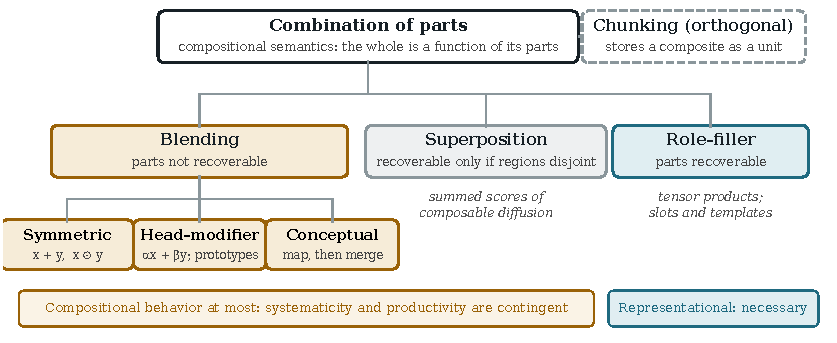
\includegraphics[width=\linewidth]{fig_taxonomy.pdf}
  \caption{A taxonomy of modes of combination. Every mode satisfies the colloquial definition, but only role--filler composition makes its parts recoverable and so satisfies Definition~\ref{def:formal}. The other modes can produce compositional behavior at most. Chunking is orthogonal.}
  \label{fig:taxonomy}
\end{figure}

\subsection{What the Definition Accounts For}
\label{sec:consequences}

A definition of compositionality should account for the properties
that motivated the concept. Appendix~\ref{app:proofs} proves six
elementary results, which show that ours accounts for systematicity as
recoverability across roles and for productivity as recoverability
across depth, and that blending accounts for neither.

\begin{enumerate}[leftmargin=*]
  \item {\it Role collisions\/} (Proposition~\ref{prop:blend}). If
  $g_r(a, b) = g_r(b, a)$ for some $a \neq b$, no readout can tell which
  part occupies which role.
  \item {\it Non-identifiability\/} (Proposition~\ref{prop:fiber}). A
  linear blend into a space smaller than its parts assigns every
  composite an affine family of decompositions. For a sum, these are
  all pairs $(x, z - x)$, so no readout, however strong, recovers the
  parts. A finite vocabulary can make parts decodable, but this
  recoverability comes from the data rather than the relation, and it
  fails for new parts.
  \item {\it Substitutivity\/} (Proposition~\ref{prop:separable}). Under
  a separable relation, a connected set of as few as $2V - 1$ observed
  pairs determines all $V^2$ composites, whereas under an unrestricted
  relation, observed composites constrain no unobserved one.
  \item {\it Systematicity as a necessary consequence\/}
  (Proposition~\ref{prop:systematic}). Under a separable and invertible
  relation, every reversal and substitution is determined by observed
  composites, whatever the training data. Without such a relation,
  systematic behavior is contingent on training in the sense of
  \citet{fodor1990} and \citet{aizawa2003}.
  \item {\it Productivity\/} (Proposition~\ref{prop:depth}). For a nested
  linear blend, the ambiguity grows as $(2^n - 1)d$ with depth $n$,
  whereas an invertible relation recovers every leaf in $n$ readouts.
  We follow \citet{fodor1988} in treating the resource limits of any
  finite implementation as matters of performance.
  \item {\it Dissociation of content and context\/}
  (Proposition~\ref{prop:context}). Under a separable relation, a part's
  learned contribution does not depend on the co-parts with which it was
  observed, so it enters new combinations without their features.
\end{enumerate}

\noindent
These results connect the definition to practical capacities.
Table~\ref{tab:cases} lists eight, each with the guarantee it requires
and evidence that current networks lack it or possess it only for
familiar combinations; Appendix~\ref{app:cases} discusses each in
detail.

\begin{table}[t]
  \caption{Capacities that depend on recoverability (details in Appendix~\ref{app:cases}).}
  \label{tab:cases}
  \centering\small
  \begin{tabularx}{\linewidth}{@{}P{3.1cm}P{3.4cm}Y@{}}
    \toprule
    Capacity & Guarantee required & Evidence of deficit in networks \\
    \midrule
    1. Who did what to whom & Distinct role reversals (Prop.~\ref{prop:blend}) & \citet{conwell2022} \\
    2. Known part, new role & Separability (Prop.~\ref{prop:separable}) & \citet{lake2018}; \citet{li2023slog} \\
    3. Reasoning about constituents & Invertibility (Prop.~\ref{prop:fiber}) & \citet{press2023}; \citet{dziri2023} \\
    4. Editing one part & Localism (Prop.~\ref{prop:systematic}) & \citet{rassin2022}; \citet{cohen2024} \\
    5. New contexts & Content--context dissociation (Prop.~\ref{prop:context}) & \citet{geirhos2020}; \citet{kamb2025} \\
    6. Arbitrary depth & Invertibility at every level (Prop.~\ref{prop:depth}) & \citet{lake2018}; \citet{dziri2023} \\
    7. New parts, no forgetting & Shared role-indexed procedure & \citet{mccloskey1989} \\
    8. Explaining outputs & Recoverable parts (Prop.~\ref{prop:fiber}) & \citet{koh2017}; \citet{grosse2023} \\
    \bottomrule
  \end{tabularx}
\end{table}

%=====================================================================
\section{Testing Recoverability}
\label{sec:tests}

The definition is useful only if it can be tested. In this section, we
describe a suite of tests, a reference profile of human performance,
and the systems we plan to evaluate. We describe the design only, and
Appendix~\ref{app:protocol} gives the full protocol and controls.

\subsection{A Test Suite}

\paragraph{Domain.} A small synthetic domain (Figure~\ref{fig:domain})
contains $V$ abstract glyphs and host frames with two roles, under two
relations. Under \textsc{beside}, parts occupy disjoint regions and
superposition suffices. Under \textsc{part-of}, a part lies within a
role region of a host, so regions overlap and a sum of parts is no
longer invertible.

\begin{figure}[t]
  \centering
  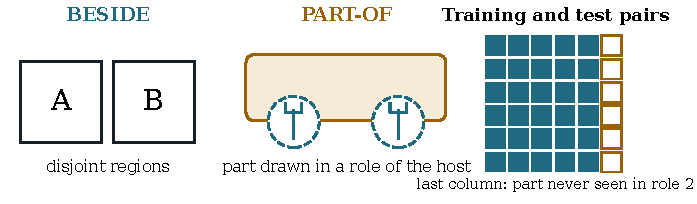
\includegraphics[width=0.85\linewidth]{fig7_test_domain.pdf}
  \caption{The test domain. \textsc{beside} places parts in disjoint regions; \textsc{part-of} places a part within a role of a host. Right: training pairs (filled) and test pairs (outlined), in which a part is never observed in role 2.}
  \label{fig:domain}
\end{figure}

\paragraph{Calibration.} The central test constructs composites
analytically with each operator of Figure~\ref{fig:taxonomy}, trains
linear, nonlinear, and nearest-neighbor readouts to recover each part,
and evaluates them on both familiar and freshly drawn parts. Only the
second condition isolates the guarantee of the relation, since it
removes the recoverability that a finite vocabulary supplies. The
resulting recovery profiles serve as references against which the
internal states of any system can be placed.

\paragraph{Tests.} Table~\ref{tab:experiments} lists seven tests, each
applied to the parts specified by the domain and to parts discovered
without supervision by a declared class $\mathcal{M}$ of methods. A
system lacks representational compositionality only if it fails under
both. Two tests go beyond accuracy. Test 3 measures context leakage,
the appearance of features from the hosts with which a part was trained
in its composites with new hosts. Test 5 measures the variance of
systematic behavior across training seeds, since behavior that is
contingent on training should vary across them, whereas behavior that
is necessary should not.

\begin{table}[t]
  \caption{The test suite (full designs in Appendix~\ref{app:protocol}).}
  \label{tab:experiments}
  \centering\small
  \begin{tabularx}{\linewidth}{@{}P{0.3cm}P{2.4cm}YY@{}}
    \toprule
    & Property; capacity & Principal manipulation & Principal measures \\
    \midrule
    1 & Recoverability; 3, 6, 8 & Analytic operators and systems; familiar and novel parts & Recovery of each part by several readouts \\
    2 & R1 & Specified and discovered parts & Recovery from internal states \\
    3 & R2, R3; 1, 2, 4, 5 & Unseen pairs, reversals, interventions, new hosts & Accuracy, error type, context leakage \\
    4 & R4; 6 & Depth beyond training & Accuracy and error type by depth \\
    5 & Contingency & Coverage, data scale, vocabulary, seeds & Data exponent; variance across seeds \\
    6 & New parts; 7 & A new part after training & Transfer; change on prior composites \\
    7 & Output form & Symbolic, image, and slot outputs & Accuracy by output type \\
    \bottomrule
  \end{tabularx}
\end{table}

\subsection{A Human Reference Profile}

We use human performance, drawn from the existing literature, as the
reference against which systems are judged. Our definition requires
evidence from internal states, which we cannot obtain from people with
probes, so we rely instead on converging evidence of two kinds. Neural
decoding shows that people represent the parts of composites
separately and reuse them, and behavioral studies show signatures that
only recoverable composition predicts, such as errors that misplace
whole parts, one-shot use of a part in a new role, and recall of parts
from learned composites. Table~\ref{tab:human} summarizes the profile.
It also records where people fall short of recoverable composition, so
that systems are not held to a standard that humans themselves do not
meet.

\begin{table}[t]
  \caption{A human reference profile drawn from the literature.}
  \label{tab:human}
  \centering\small
  \begin{tabularx}{\linewidth}{@{}P{3.3cm}YP{2.9cm}@{}}
    \toprule
    Signature & Human evidence & Sources \\
    \midrule
    Separate codes for roles & Agent and patient decoded from separate regions, generalizing across verbs & \citet{frankland2015} \\
    Composition of known parts & Novel objects represented and inferred as compositions of known elements & \citet{schwartenbeck2023} \\
    Known part, new role & A newly learned word applied correctly in unseen combinations & \citet{lake2019} \\
    Parts kept within chunks & Expert recall organized by chunks and templates with recoverable parts & \citet{chase1973}; \citet{gobet2000} \\
    Form-based inference & Valid inferences endorsed across arbitrary contents; logical concepts learned as compositions & \citet{rips1994}; \citet{piantadosi2016} \\
    Limits & Belief overrides validity; content alters selection; concepts often blended & \citet{evans1983}; \citet{wason1968}; \citet{wisniewski1997} \\
    \bottomrule
  \end{tabularx}
\end{table}

\subsection{Systems to Evaluate}

We plan to evaluate two groups of systems with the suite. The first
contains deliberately simple neural networks, namely multilayer
perceptrons, small convolutional networks, and small transformers
trained from scratch with at least ten seeds, chosen so that every
internal state can be examined and so that no composition can be
attributed to uncontrolled pretraining. The second contains existing
systems that build in parts of the criterion: tensor product and
holographic reduced representations \citep{smolensky1990,plate1995},
slot-wise decoders, which provably generalize to unseen slot
combinations under additivity \citep{wiedemer2024}, DORA, which learns
relations from unstructured input \citep{doumas2022}, CHREST
\citep{gobet2000}, and \textsc{Trellis}, which records for every element
both what it is made of and how it behaves \citep{singaravadivelan2026}.
\note{Insert the initial results of TRELLIS here, if any are to be reported.}
We classify each system and relation into three grades fixed in
advance, following Table~\ref{tab:twobytwo}. A system that fails the
behavioral criteria blends, one that meets them without a decomposition
under $\mathcal{M}$ imitates composition, and one that meets all
criteria is representationally compositional for the relation tested.

%=====================================================================
\section{Related Work}
\label{sec:related}

Our account builds most directly on \citet{vegner2025}, who distinguish
behavioral from representational systematicity, sort existing
benchmarks by Hadley's levels, and recommend mechanistic
interpretability as the route to representational claims. We share
their distinction and supply a criterion for its representational side.
\citet{hupkes2020} decompose compositional generalization into
behavioral tests, and our tests add measures of internal recoverability
to theirs. \citet{elmoznino2024} define representational
compositionality by description length, and \citet{elmoznino2026}
measure the compositional structure of objects by the information that
a whole adds beyond its parts. Both are compression-based, and neither
requires that parts be recoverable, so a blend could score well under
them and fail under ours. \citet{andreas2019} estimate how closely an
explicit composition of primitives reproduces a representation, which
corresponds to our separability without invertibility. On the side of
the classical debate, \citet{goodale2026} argue that the systematicity
challenge concerns what an architecture guarantees, and
\citet{woydt2025} argue that meta-learning has not yet produced
human-like systematic compositionality. Our results give a formal
version of the first claim and a way of testing the second.

Two objections deserve brief replies. The first, due to
\citet{fodor1990}, is that recoverability is not enough because
constituents must be tokened to cause systematic processing. Our reply
is that the necessity they wanted comes from the relation: when one
invertible relation serves every filler and role, the ability to handle
any composite follows from the ability to handle one. The second is
that the requirement of extractability is unfalsifiable, since a
negative result can be blamed on weak methods. We therefore require
that methods be declared in advance and validated on systems with known
decompositions, and Proposition~\ref{prop:fiber} ensures that no method
will find parts that a relation has discarded.

%=====================================================================
\section{Concluding Remarks}
\label{sec:conclusion}

In this paper, we proposed a recoverability-based theory of
compositionality. We defined representational compositionality as
combination through a relation from which every part can be recovered
in its role, showed that this definition accounts for systematicity,
productivity, and the dissociation of content from context, and
showed that blending accounts for none of them. We then described a
suite of tests, a human reference profile, and a plan for evaluating
networks and structured systems. One implication concerns terminology:
behavioral evidence should be reported as compositional generalization,
and the bare term should be reserved for systems whose parts have been
shown to be recoverable. Several questions remain open:

\begin{itemize}
  \item Can unsupervised methods reliably discover the primitives of a
  network, so that a negative result reflects the network rather than
  the method?
  \item Does any training regime, or any increase in scale, lead a
  network without built-in roles to representational composition under
  overlapping roles?
  \item Can a system keep its parts recoverable while matching neural
  networks in perception and graded similarity?
\end{itemize}

\bibliographystyle{plainnat}
\bibliography{references}

%=====================================================================
\clearpage
\appendix

\section{Formal Results}
\label{app:proofs}

This appendix states and proves the results summarized in
Section~\ref{sec:consequences}. Throughout, we use the notation of
Eq.~\eqref{eq:binding}.

\begin{figure}[h]
  \centering
  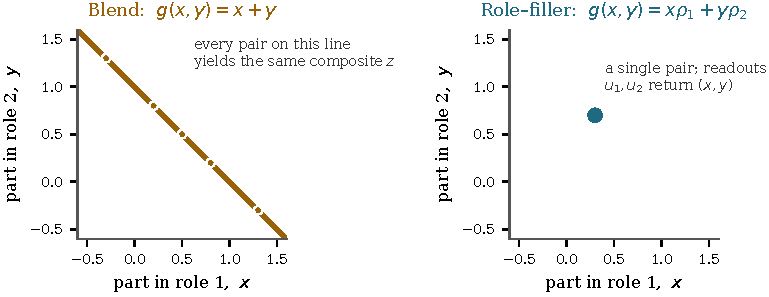
\includegraphics[width=0.78\linewidth]{fig_fibers.pdf}
  \caption{Non-identifiability of blended parts (Proposition~\ref{prop:fiber}), shown for scalar parts. Under $x + y$, every pair on the line yields the same composite; under a role--filler relation, each composite has one decomposition.}
  \label{fig:fibers}
\end{figure}

\begin{proposition}[Role collisions]
\label{prop:blend}
If $g_r$ is not injective under exchange of roles, so that $g_r(a, b) = g_r(b, a)$ for some parts $a \neq b$, then no readout of $\rep(c)$ can determine which of $a$ and $b$ occupies which role. In particular, every symmetric relation fails R2 for every such pair, and no non-invertible relation satisfies R1.
\end{proposition}

\begin{proof}
By Eq.~\eqref{eq:binding}, $\rep(r(a, b)) = \rep(r(b, a))$, and any readout of identical representations returns identical values. If $g_r$ is not invertible, distinct tuples of parts share a representation by definition, and no readout distinguishes them.
\end{proof}

\begin{proposition}[Non-identifiability of blended parts]
\label{prop:fiber}
Let the representations of parts lie in $\R^d$, and let $g_r(x_1, \ldots, x_k) = \sum_{i} A_i x_i \in \R^m$ with matrices $A_i \in \R^{m \times d}$, so that symmetric blending, weighted addition, and superposition are special cases. If $\mathrm{rank}\,[A_1 \cdots A_k] < kd$, which holds whenever $m < kd$ and hence for every blend into the space of its parts, then for every composite $z$ in the image of $g_r$ the set of tuples with $g_r(x_1, \ldots, x_k) = z$ is an affine subspace of dimension $kd - \mathrm{rank}\,[A_1 \cdots A_k] \geq 1$. No readouts $u_i$, linear or nonlinear, recover the parts of every composite.
\end{proposition}

\begin{proof}
Write $A = [A_1 \cdots A_k]$ and $t = (x_1, \ldots, x_k) \in \R^{kd}$, so that $g_r(t) = At$. If $At_0 = z$, the solutions of $At = z$ are $t_0 + \ker A$, and $\dim \ker A = kd - \mathrm{rank}\, A \geq 1$ by the rank--nullity theorem. Any nonzero $n \in \ker A$ has a nonzero block $n_i$, so the tuples $t_0$ and $t_0 + n$ share the composite $z$ but differ in their $i$-th part, and no function of $z$ returns the $i$-th part of both.
\end{proof}

\begin{remark}
The result extends beyond linear relations, since no continuous map from $\R^{kd}$ to $\R^m$ with $m < kd$ is injective. When parts come from a finite vocabulary, a non-invertible relation may happen to be injective on that vocabulary, and the parts can then be decoded. In that case, recoverability comes from the sparsity of the vocabulary rather than from the relation, so it fails for parts outside the vocabulary and degrades as the vocabulary grows relative to $m$. A tensor product representation with linearly independent roles has $\mathrm{rank}\, A = kd$ and recovers the parts of every composite, including composites of parts never seen before.
\end{remark}

\begin{proposition}[Substitutivity]
\label{prop:separable}
Let $r$ be binary and separable with $\psi = \mathrm{id}$, so that $g_r(x, y) = \varphi_1(x) + \varphi_2(y)$, and let $O$ be a set of observed pairs whose bipartite graph, with fillers of role 1 and of role 2 as vertices and observed pairs as edges, is connected. Then the values of $g_r$ on $O$ determine its value on every pair $(x, y)$ of vertices, including pairs never observed together. If $g_r$ is unrestricted, its values on $O$ place no constraint on any unobserved pair.
\end{proposition}

\begin{proof}
For any edges $(x, y'), (x', y'), (x', y) \in O$, separability gives $g_r(x, y) = g_r(x, y') - g_r(x', y') + g_r(x', y)$. Connectivity lets us chain this identity along a path from $x$ to $y$, so $g_r(x, y)$ is determined. The functions $\varphi_1$ and $\varphi_2$ are determined only up to opposite constant shifts, which cancel in every value of $g_r$. For an unrestricted $g_r$, the value at an unobserved pair can be set independently of all observed values.
\end{proof}

\begin{proposition}[Systematicity as a necessary consequence]
\label{prop:systematic}
Let $r$ be separable and invertible. Then (i) for any parts $a \neq b$, the composites $g_r(a, b)$ and $g_r(b, a)$ are distinct; (ii) replacing the part in role $i$ changes $\psi(g_r)$ only in the term $\varphi_i$ and leaves every readout $u_j$, $j \neq i$, unchanged; and (iii) under the conditions of Proposition~\ref{prop:separable}, every role reversal and every substitution of an observed filler into an observed role is determined by the observed composites.
\end{proposition}

\begin{proof}
(i) Invertibility gives $u_1(g_r(a, b)) = a \neq b = u_1(g_r(b, a))$, so the composites differ. (ii) By separability, $\psi(g_r)$ is a sum in which only $\varphi_i(x_i)$ depends on $x_i$, and by invertibility $u_j$ returns $x_j$, which has not changed. (iii) A reversal $(b, a)$ and a substitution $(x, y)$ are pairs of vertices of the observed graph, and Proposition~\ref{prop:separable} applies to each.
\end{proof}

\noindent
Proposition~\ref{prop:systematic} is the formal version of the
necessity that \citet{fodor1990} demanded. Under a separable and
invertible relation, the ability to build and read one composite
entails the ability to build and read its reversal and its
substitutions, whatever the training data. Under an unrestricted
relation, observed composites place no constraint on unobserved ones,
so any systematic behavior on them depends on training and is in this
sense contingent \citep{aizawa2003}.

\begin{proposition}[Productivity requires recoverability at every level]
\label{prop:depth}
Let $g(x, y) = Ax + By$ with $A, B \in \R^{d \times d}$, so that composites lie in the same space as their parts and can serve as parts. A balanced composite of depth $n$ has $2^n$ primitive leaves, and the map from the leaves to the composite has a kernel of dimension at least $(2^n - 1)d$. If instead the relation at each level is invertible, every leaf can be recovered by $n$ successive readouts.
\end{proposition}

\begin{proof}
The map from the leaves, which lie in $\R^{2^n d}$, to the composite in $\R^d$ is a composition of linear maps and so is linear, with rank at most $d$. By rank--nullity, its kernel has dimension at least $2^n d - d$. If each level is invertible, readouts at the root return the two subcomposites, and applying readouts recursively returns every leaf after $n$ steps.
\end{proof}

\noindent
No representation of fixed size can invertibly encode trees of
unbounded depth over continuous parts. Tensor products grow in
dimension with depth, and holographic reduced representations
accumulate noise \citep{smolensky1990,plate1995}. We follow
\citet{fodor1988} in treating such limits as matters of performance:
the relation guarantees recoverability at every depth in principle,
and finite resources bound how far an implementation can go.

\begin{proposition}[Dissociation of content and context]
\label{prop:context}
Under the conditions of Proposition~\ref{prop:separable}, the contribution $\varphi_1(x)$ of a filler $x$ that is determined by the observed composites does not depend on which of its co-parts were used to determine it, and it is the same, up to a constant common to all fillers of its role, for any connected set of observations containing $x$. If $g_r$ is unrestricted, the composites observed with $x$ place no constraint on its contribution in combination with any other part.
\end{proposition}

\begin{proof}
For every $y$ observed with $x$, separability gives $\varphi_1(x) = g_r(x, y) - \varphi_2(y)$, and $\varphi_2$ is determined up to a constant by the connected graph (Proposition~\ref{prop:separable}). The identity holds for each such $y$, so every choice of co-part yields the same value of $\varphi_1(x)$, and the constant is fixed by a single normalization of the role. For an unrestricted $g_r$, the value at an unobserved pair is free, as in Proposition~\ref{prop:separable}.
\end{proof}

\noindent
Proposition~\ref{prop:context} extends the classical requirement that a
constituent contribute the same thing to every whole, from the wholes
in which a part is used to the wholes from which it was learned. The
connectionist reply to the classical argument explicitly accepted
context-dependent constituents \citep{smolensky1987}, and the prototype
literature concedes that prototype combination is not compositional in
the strict sense, because emergent attributes draw on general
knowledge \citep{hampton2012,osherson1981,fodor1996}.

\section{Modes of Combination}
\label{app:forms}

Table~\ref{tab:forms} gives an exemplar relation and sources for each
mode in Figure~\ref{fig:taxonomy}. In the selective modification model,
the modifier changes the values and weights of those attributes of the
head to which it applies \citep{smith1988}, and in composite
prototypes, attribute conflicts are resolved and emergent attributes
appear according to the particular pair combined \citep{hampton1987}.
Language models mostly fail at the mapping step of conceptual blending
\citep{schapiro2025}. Holographic reduced representations satisfy both
separability and invertibility approximately \citep{plate1995}.

\begin{table}[h]
  \caption{Modes of combination, distinguished by the properties of the relation $g_r$.}
  \label{tab:forms}
  \centering\small
  \begin{tabularx}{\linewidth}{@{}P{2.4cm}P{2.7cm}P{1.3cm}P{1.6cm}YP{2.2cm}@{}}
    \toprule
    Mode & Exemplar $g_r$ & Distinct roles & Separable & Invertible & Sources \\
    \midrule
    Symmetric blending & $x + y$; $x \odot y$ & No & Yes; $x \odot y$ under $\log$ & No & \citet{mitchell2010} \\
    Head--modifier blending & $\alpha x + \beta y$; selective modification; composite prototypes & Yes & Only for weighted addition & No & \citet{mitchell2010}; \citet{smith1988}; \citet{hampton1987} \\
    Superposition & Sum of representations & By region only & Yes & Only if regions are disjoint & \citet{liu2022composable} \\
    Conceptual blending & Structural mapping, then integration & Partially & No & Partially & \citet{fauconnier2002} \\
    Role--filler composition & $\sum_i x_i \otimes \rho_i$ & Yes & Yes & Yes & \citet{smolensky1990}; \citet{plate1995} \\
    \bottomrule
  \end{tabularx}
\end{table}

\section{Capacities That Depend on Recoverability}
\label{app:cases}

\paragraph{Case 1: Telling who did what to whom.} A system that
represents a relation must distinguish a composite from its role
reversal (Proposition~\ref{prop:blend}). This is important whenever
roles carry the meaning, as in an instruction to move one object onto
another or a report that one drug inhibits the metabolism of another.
People encode agent and patient in separate codes \citep{frankland2015},
whereas text-to-image models matched about 22 percent of prompts
describing fifteen basic relations in one evaluation \citep{conwell2022},
and summing separately conditioned scores works when objects occupy
separate regions but not when one must occupy a region of another
\citep{liu2022composable,anonymous2026seen}.

\paragraph{Case 2: Using a known part in a new role.} A separable
relation guarantees that a part seen in one role can be used in another
(Proposition~\ref{prop:separable}). This is important because a learner
sees only a small fraction of the combinations it must handle. On the
structural cases of SLOG, transformers reached at most 40.6 percent
while performing near ceiling when a new word appeared in a familiar
frame \citep{li2023slog}, a failure of strong systematicity in
\citeauthor{hadley1994}'s (\citeyear{hadley1994}) sense.

\paragraph{Case 3: Reasoning about constituents.} Inference that is
sensitive to structure must find constituents within the whole
(Proposition~\ref{prop:fiber}), and an error at any step of a chain
reaches its conclusion. Language models answer the sub-questions of a
compositional question more often than the question itself
\citep{press2023}, and transformer accuracy declines with the depth of
the computation \citep{dziri2023}.

\paragraph{Case 4: Editing one part without disturbing the others.} A
separable and invertible relation lets a system replace one part while
leaving the readouts of the others unchanged
(Proposition~\ref{prop:systematic}). This is important for controllable
generation and for updating knowledge. Text-to-image models often
express an attribute named for one object on another
\citep{rassin2022,huang2023t2i}, and edits to one fact in a language
model fail to propagate consistently to the facts that depend on it
\citep{cohen2024}.

\paragraph{Case 5: Carrying a part into a new context.} A part learned
in some contexts should enter new combinations without their features
(Proposition~\ref{prop:context}). Networks often rely on features of the
training context that are correlated with, but not part of, the
content \citep{geirhos2020}, and convolutional diffusion models produce
novel images as mosaics of training patches \citep{kamb2025}. In the
hippocampal formation, by contrast, a model that separates the
structure of an environment from its sensory content transfers that
structure to new environments \citep{whittington2020}.

\paragraph{Case 6: Composing to arbitrary depth.} An invertible
relation at every level lets a system build and interpret structures
deeper than any it has seen (Proposition~\ref{prop:depth}), as nested
instructions, programs, and plans require. On the SCAN split that
requires longer outputs, the best networks of 2018 reached 20.8 percent
\citep{lake2018}, and errors in multi-step computation compound with
depth \citep{dziri2023}.

\paragraph{Case 7: Acquiring new parts without forgetting.} With a
shared role-indexed procedure, a new primitive is a single act of
learning that alters no stored part. When combinations are encoded in
shared weights, each new combination is a separate learning problem,
and updating the weights interferes with what was learned before
\citep{mccloskey1989,french1999}.

\paragraph{Case 8: Explaining an output by its parts.} A system whose
composites retain their parts can explain an output by the parts it
reused. Training data attribution traces outputs to influential
examples \citep{koh2017,grosse2023}, but it does not identify which
parts an output reuses, and by Proposition~\ref{prop:fiber} a blended
representation does not determine them.

\section{Experimental Protocol}
\label{app:protocol}

\paragraph{Criteria.} Each criterion is stated relative to the
network's own performance on a difficulty-matched baseline of randomly
withheld combinations whose filler--role pairs all appeared in
training. A criterion is met when performance on structurally novel
items lies within five percentage points of that baseline, when errors
preserve the identity of parts, and when interventions on a part alter
only its role. Networks are trained at three sizes. Each composite is
presented as a symbol string, an image, and a sentence.

\paragraph{Experiment 1: Recoverability of parts.} In a calibration
stage, we construct composites analytically with each operator in
Table~\ref{tab:forms} over Gaussian part vectors, varying the ratio of
representation to part dimension, the vocabulary size $V$, and the
depth of nesting. We train linear probes, multilayer perceptron probes,
and nearest-neighbor decoders to recover the part in each role and
evaluate them on composites of training parts and of freshly drawn
parts. In a network stage, we apply the same readouts to each layer,
with shuffled-label control tasks \citep{hewitt2019}, and also over
primitives discovered by sparse dictionary learning, so that a failure
due to the level of primitives is not mistaken for a failure of the
relation. A finding that parts are recoverable only for familiar
vocabularies would show that apparent constituent structure comes from
the data rather than from the relation.

\paragraph{Experiment 2: Constituent structure (R1).} We train a linear
probe for each role on frozen states and apply the methods in
$\mathcal{M}$ to the same states, measuring recovery on baseline and
held-out composites under both relations and both decompositions.

\paragraph{Experiment 3: Substitution, reversal, and context (R2, R3).}
We withhold every pair in which a part occupies role 2, test
role-reversed items, and apply interchange interventions that swap the
internal representation of one part for that of another. We measure
accuracy, the classification of errors as whole-part misplacements or
blends, and the fraction of each intervention's effect confined to its
role. We also test Proposition~\ref{prop:context} by measuring whether
a part's recovered representation stays stable across hosts and
whether features of its training hosts appear in its composites with
new hosts, and we ask whether success at reversal comes with the
recoverability measured in Experiment 1.

\paragraph{Experiment 4: Depth (R4).} We train on depths one and two,
test on depths three to five, and measure accuracy and error type by
depth.

\paragraph{Experiment 5: Contingency and data.} We vary the proportion
of filler--role pairs observed, the amount of data, and the vocabulary
size from 8 to 64. We estimate the exponent $\beta$ in the data
requirement $N^{*}(V) \propto V^{\beta}$, with $\beta \approx 1$, the value for a system with a shared
role-indexed procedure, as a reference, and the variance of systematic
behavior across seeds and data orderings.

\paragraph{Experiment 6: A new primitive (lifelong learning).} We
introduce a new part with five examples in a single host and role,
with and without replay, and measure transfer to other hosts and roles
and the change in performance on prior composites.

\paragraph{Experiment 7: Output form.} We train one encoder with a
symbolic decoder, an image decoder, and a decoder with one slot per
part, to determine whether failures arise in the representation or in
the form of the output.

\begin{table}[h]
  \caption{Threats to validity and the corresponding controls.}
  \label{tab:controls}
  \centering\small
  \begin{tabularx}{\linewidth}{@{}YY@{}}
    \toprule
    Threat to validity & Control \\
    \midrule
    The network composes over parts the experimenter did not specify & Every property is also tested against discovered parts under $\mathcal{M}$ \\
    Failure to find a decomposition reflects the methods, not the network & $\mathcal{M}$ is declared in advance and validated on the analytic operators of Experiment 1, tensor product representations, and networks with built-in slots \\
    Recovery reflects a memorized vocabulary rather than the relation & Readouts are evaluated on freshly drawn parts as well as on training parts \\
    Held-out items are harder rather than structurally different & A difficulty-matched baseline of randomly withheld pairs \\
    The criteria cannot be met by any learner & Systems with built-in recoverable relations are run on every test \\
    Probes detect what they are trained to detect & Shuffled-label control tasks \citep{hewitt2019} \\
    Seed variance; scale & At least ten seeds; three sizes per architecture \\
    \bottomrule
  \end{tabularx}
\end{table}

\end{document}
